\documentclass{report}
\usepackage{graphicx} % Required for inserting images
\usepackage{url}
\usepackage{biblatex}
\usepackage{rotating}
\graphicspath{ {./images/} }
\title{Project Proposal}
\author{Otito Mbelu (G00397738)}
\date{\today}

\addbibresource{biblio.bib}

\begin{document}
\setlength{\parindent}{0pt}
\maketitle

\chapter*{Project Proposal}
    \textbf{Supervisor:} Dr. Damien Costello \par
    \textbf{Project Name:} Biometric Data Analysis in Digital Game Scenario
    \section*{Project Context}
    \subsection*{Introduction}
    \par
    \textbf{PUBG:} Battlegrounds (previously known as PlayerUnknown\'s Backgrounds) is a battle royale style player versus
    player shooter game developed by PUBG Studio. Players face-off with each other using various types of battlefield weapons
    in a last man standing deathmatch and the last person to remain alive wins. The game is available in all major platforms
    and as of March 2021, the mobile version of the game has accumulated more than a billion download outside of China with 
    revenue of over \$9billion while the PC and console versions have accumulated a total revenue of \$4billion
    \cite{statista}.
    \par 
    Since its first release in 2017, the game has since become one the fans favorite and has over `350,000' peak concurrent 
    monthly users~\cite{statista}. As a multiple award-winning game with proven longevity records and a large community.
    Interest in the game cut across diferent demography and is equally far-reaching across the globe. 
    The game playing scenario requires players to face-off with other players and there is where some skills like 
    `eye-hand-coordination', `ear-hand-codination', `fine-motor' skills, etc\.. are required to compete favorably against 
    other players. Players have access to ora varieties of weapons with different capabilities and can make in-game adjustments
    to their control to suite their various preferences. 
    This project is a continuation of research work previously done by Fourth Year Software Design Students titled `Biometric 
    Data Collection for Performance Optimization in a Digital Game Scenario' in collaboration with the Department of Sports
     \& Excercise Science, Atlantic Technological University.
    \subsection*{Previous Projects}
    The originiating project titled \textbf{`Biometric Data Collection for Performance Optimization in a Digital
    Game Scenario'}, posed the question `can a player\'s biometrica data be used to optimise their performance in a 
    first-person shooter game'? And a subsequent follow up project which sought to create a Chart API capable of displaying 
    all relevant information previously displayed on different pages on a single page.\\
    The former research was geared towards creating a test environment where players can 
    practice and horn their skills in a similar scenarios (Weapons, controls, user perspective, ect\..) obtainable in PUBG\:: 
    Battlegrounds in the form of a Unity Desktop {\tt Application}. Collection and storage of Biometric data from an 
    {\tt Activity Monitor} in the form of a {\tt Smart Watch}. With the enventual goal of finding correlation between their
    performance and their Biometric data. 
    \\

    
    \section*{Project Objective}
        The objective of this research project will seek to address some of the limitation listed in the previous projects and
        complete the future development goals of both projects. 
        These includes\::
        \begin{itemize}
            \item{Chart API Integration}: Integrating the developed Chart API into the Test Application.
            \item {Offline Data Storage}: Provision will be made for offline temporary file storage to improve the overall 
            reliability of the whole system
            \item{PUBG API}: Further research on new developments in the PUBG API for better user experience. 
        \end{itemize} 
        
        And eventually seek to answer the following research questions\::

        \begin{itemize}
            \item {Can users' current physical condition as indicated by their Biometric data, have any direct relationship with 
            their performance in such gaming scenario?}
            \item {Can Biometric and test data help suggest the most suitable settings for different game scenarios?}
        \end{itemize}


    \section*{Technologies \& System Architecture}
    \subsection*{Legacy Architecture}

        The overall system architecture is depicted in Figure~\ref{fig:architecture}. The system is made up of three modules 
        interacting with an external API and user devices. The modules are listed as follows:
        \begin{itemize}
            \item{Test Application} A Unity designed desktop application on Windows Platform that where users can play test 
                for different game scenarios.
            \item {Node Js Web Application}
                An Express Node JS Web application deployed on Amazon EC2 Virtual machine, serving as a callback endpoint for 
                OAuth 2.0 Authentication for the Polar Flow API. 
            \item {Firestore Data Storage}
                Permanent storage medium for users' test and Biometric data.
        \end{itemize}
        User Devices:
        \begin{itemize}
            \item{Smart Watch}
            \item {Smart Phone}
        \end{itemize}
        \begin{figure}[h]
        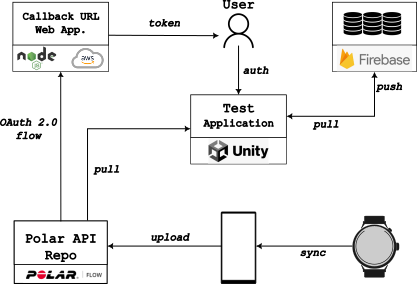
\includegraphics{images/architecture.png}
        \caption{System Architecture}
        \label{fig:architecture}
        \centering
        \end{figure}
        The actions in the Figure~\ref{fig:architecture} can be summarized as follows:
        \begin{itemize}
            \item{sync}: passing of biometric data to a smart phone from a Polar watch.
            \item {upload}: uploading of biometric data to Polar API repository.
            \item {OAuth 2.0 flow}: Multi step OAuth 2.0 authentication protocol. 
            \item {token}: getting verification token from the Callback URL by the user.
            \item {pull (Polar API - Test Application)}: retrieving biometric data from Polar API by the Test Application.
            \item {auth}: user supplies token to the Test Application as final step of authentication. 
            \item {pull (Firebase - Test Application)}: retrieving user test/biometric data for rendering by Test Application.
            \item {push}: saving users' test/biometric data to a Datastore.
        \end{itemize}
    \subsection*{Proposed Architecture}
    The final system architecture will include new modules to facilitate data analytics using A.I models. The new system calls 
    for a relational database replica of the Firebase storage to ensure data consistency, predictability and structures suitable
    for relevant statistical analysis. A.I models as a mini service that perform operations with supplied data and returns result
    of analysis. A Web Application that functions as a Controller that interfaces the data and A.I modules, Executive Dashboard 
    that renders user data, results from the A.I Modules and any other relevant information about the system.\\
    Figure~\ref{fig:proposed-web-architecture} shows the proposed architecture for the System.
    \begin{figure}[h]
        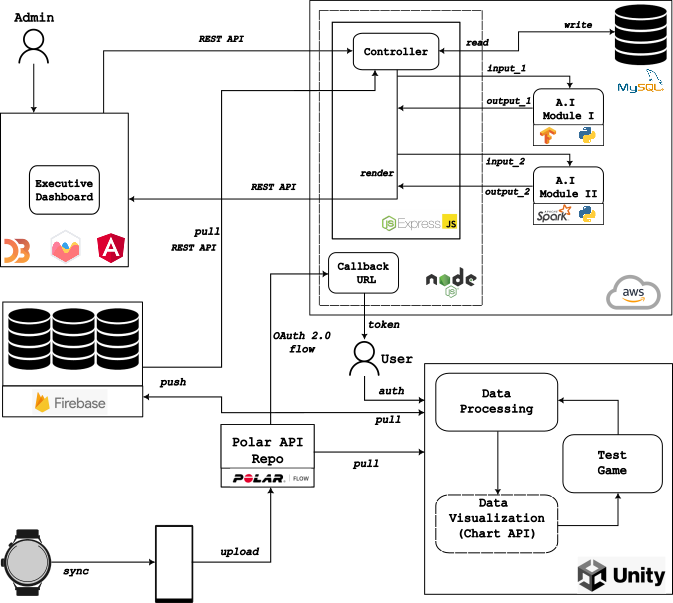
\includegraphics[scale=0.675]{images/proposed-architecture.png}
        \caption{Proposed Architecture}
        \label{fig:proposed-web-architecture}
    \end{figure}
    From the diagram above, additional modules have been added to the system which are: the back-end `Controller', front-end 
    `Executive Dashboard', a `Relational Database', and A.I Modules. The functions of these modules are explained below:
    \begin{itemize}
        \item {Controller}: This module is responsible for coordinating data fetch from the Relational Database and making sure 
        that the Relational Database is always in sync with the Firebase Datastore. It is also responsible for filtering
        and structuring data being fed into the A.I. Modules and when necessary, using the output for an A.I module as input to
        another A.I module. 
        \item{Executive Dashboard}: This module provides a Graphical User Interface that displays the working dataset, and 
        offers interfaces to filter, tune and if necessary, bias data being sent to the A.I Modules for analysis. This module will
        be developed using the Angular Framework with integration of D3.js or Chart.js for displaying relevant charts. The choice 
        for Angular Framework over other solutions namely ReactJS and Vue is because of the more structured nature of the 
        Angular Framework which is more suited for collaborative development. 
        \item{A.I Modules}: These modules are responsible for running analysis on data. The modules accepts input from the 
        `Controller' and outputs a comprehensive summary of the results of the analysis which is displayed on the 
        `Executive Dashboard' Module. For this purpose Tensorflow \& Apache Spark were chosen for the following reasons:
        \begin{itemize}
            \item{Capabilities}: Apache Spark is capable of performing linear and logical regression which are the common tools
            used for this class of problem. Tensorflow is also capable of performing the afore-mentioned techniques and can 
            perform regression using neural network models.  
            \item {Accessibility}: The both tools are open-source and available to the general public.
            \item {Python API interface}: The both tools provide a Python API. This provide ease of deployment as Python is 
            platform independent and relatively easy to setup in an Ubuntu Virtual machine. 
            \item{Large Community}: Both have large community of contributors. Documentation and tutorials are readily available 
            on the internet. 
        \end{itemize}
    \item{Relational Database}: Data for the analysis will be sourced directly from this Database which is a structured replica of
    the Firestore Database as obtained from the Legacy System. The rationale for this Module is to provide a flexible means of
    retrieving data in various forms and shape as may be needed for analysis and also overcome the high complexities involved
    in Firestore for compound queries. The MySQL Database was chosen for this purpose for the following reasons:
    \begin{itemize}
        \item{Available}: MySQL is open-source and free, thus suitable for this project. 
        \item {Secured}: Offers security with its User account management system.
        \item {Durability}: MySQL API is available for most programming language and widely used.
    \end{itemize}
    \item{REST APIs}: Communication Interface between various components of the system. The JSON format which is considered 
    standard will be used for this purpose.
    \item{Chart API}:  is responsible for displaying users' test results and biometric data to the users. This already developed 
    module will be integrated into the `Test Application' and undergo some modification to be able to display custom data as 
    requirements change.
    \end{itemize}
    
    \section*{Schedule of work}
    I will be solely responsible for the design and implementation of the Controller, The Relational Database and Tensorflow
    A.I Module. In collaboration, design the REST APIs between the Controller, Executive Dashboard, and the A.I Modules. 
    Adaptation and Integration of the Chart API into the Test Application. 
    \begin{sidewaysfigure}
        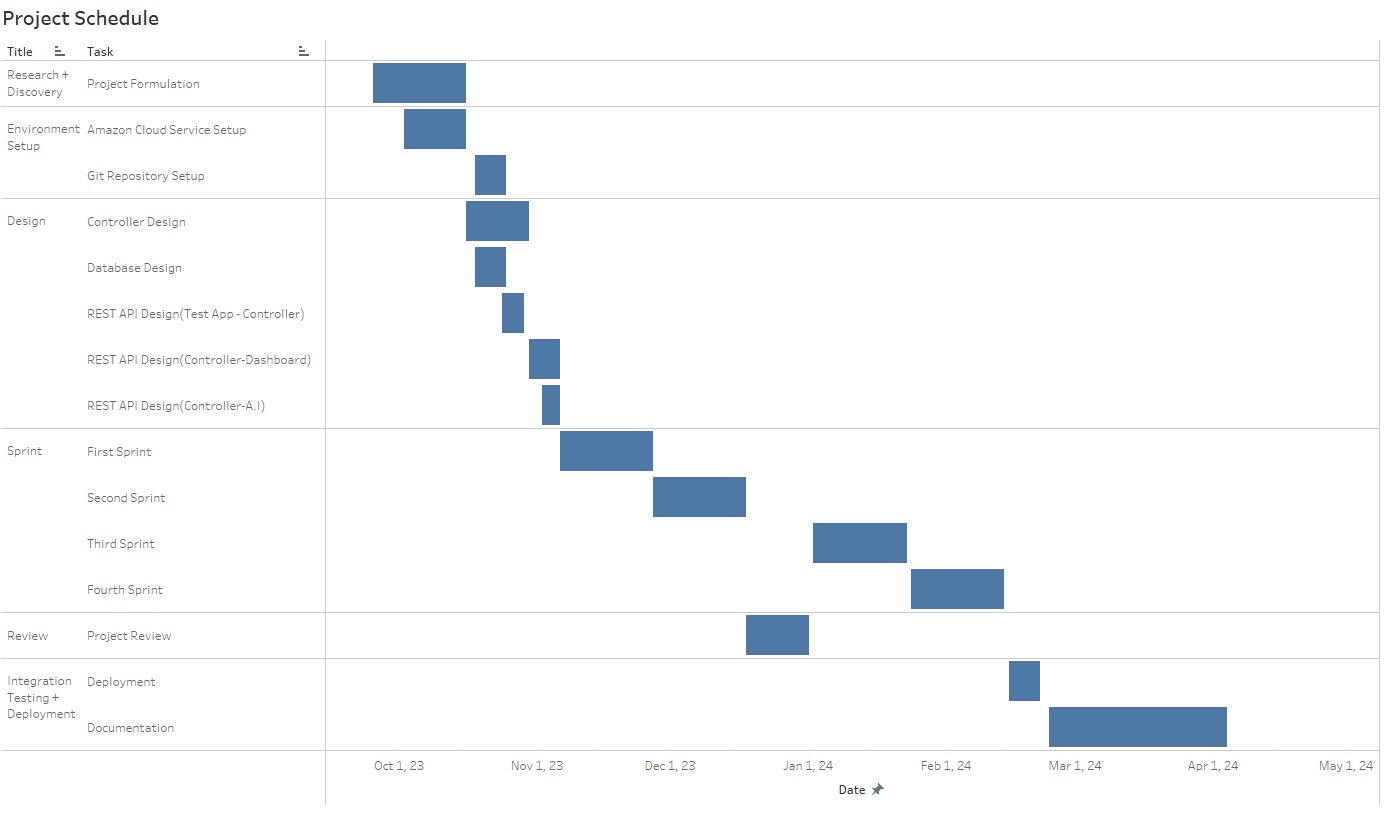
\includegraphics[scale=0.63]{images/schedule.png}
        \caption{Project Schedule}
        \label{fig:schedule}
        \centering
    \end{sidewaysfigure}
    \printbibliography


\end{document}
